\documentclass{article}
\usepackage[english]{babel}
\usepackage{amsmath}
\usepackage{newtxtext,newtxmath}
\usepackage{graphicx}
\usepackage{subcaption}
\usepackage{float}
\usepackage[margin=0.7in]{geometry}
\usepackage[utf8]{inputenc}
\usepackage{listings}
\usepackage{color}

\definecolor{dkgreen}{rgb}{0,0.6,0}
\definecolor{gray}{rgb}{0.5,0.5,0.5}
\definecolor{mauve}{rgb}{0.58,0,0.82}

\lstset{frame=tb,
  language=Java,
  aboveskip=2mm,
  belowskip=2mm,
  showstringspaces=false,
  columns=flexible,
  basicstyle={\small\ttfamily},
  numbers=none,
  numberstyle=\tiny\color{gray},
  keywordstyle=\color{blue},
  commentstyle=\color{dkgreen},
  stringstyle=\color{mauve},
  backgroundcolor=\color{gray},
  breaklines=true,
  breakatwhitespace=true,
  tabsize=3
}

\newcommand{\maximize}{%
  \mathopen{}\operatorname*{maximize}%
}

\title{Betulla Rescue \\ Interactive Graphics Project}
\author{Leonardo Brizi\\Tommaso Carlini\\Eleonora Chiarantano}

\begin{document}

\maketitle

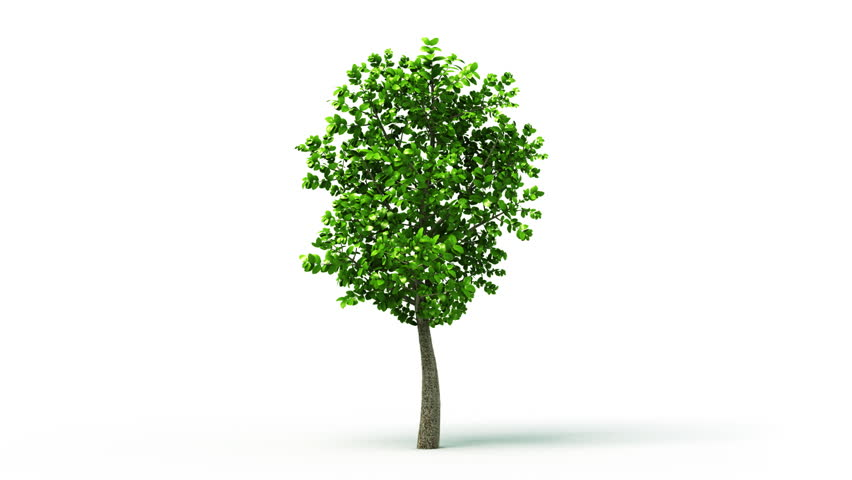
\includegraphics[width=\linewidth]{ImmaginiReport/immag.png}

\newpage

\section*{Introduction}
Betulla Rescue is the result of the collaboration of three students from La Sapienza University, with the aim of creating a game that was intuitive, fun and dealt with real issues. Within the game the player is the pilot of a Bombardier-415, better known as Canadair, an aircraft supplied to firefighters to fight large fires in areas difficult to reach. The goal is to limit and then extinguish a fire in the shortest possible time. The player will be supported during the game by the co-pilot Camil, who will provide valuable information throughout the mission, will strive to give advice on altitude, speed, commands to press and much more. The game ends when the fire is completely extinguished.

\section*{Environments}

The world and the plane were created using the library three.js\footnote{https://threejs.org} a library of Javascript used to create and display animated 3D computer graphics in a web browser. Within three.js we have subsequently imported the following libraries:
\begin{itemize}
\item \textit{dat.gui.min.js}: A lightweight graphical user interface for changing variables in JavaScript.
\item \textit{GLTFLoader.js}:glTF (GL Transmission Format) is an open format specification for efficient delivery and loading of 3D content.
\item \textit{MTLLoader.js}: The Material Template Library format (MTL) or .MTL File Format is a companion file format to .OBJ that describes surface shading (material) properties of objects within one or more .OBJ files.
\item \textit{OBJLoader.js}: The OBJ file format is a simple data-format that represents 3D geometry in a human readable format.
\item \textit{TextureLoader.js}: Class for loading a texture.
\end{itemize}

\subsection*{Models}

\subsubsection*{Bombardier-415}

\begin{figure}[h!]
  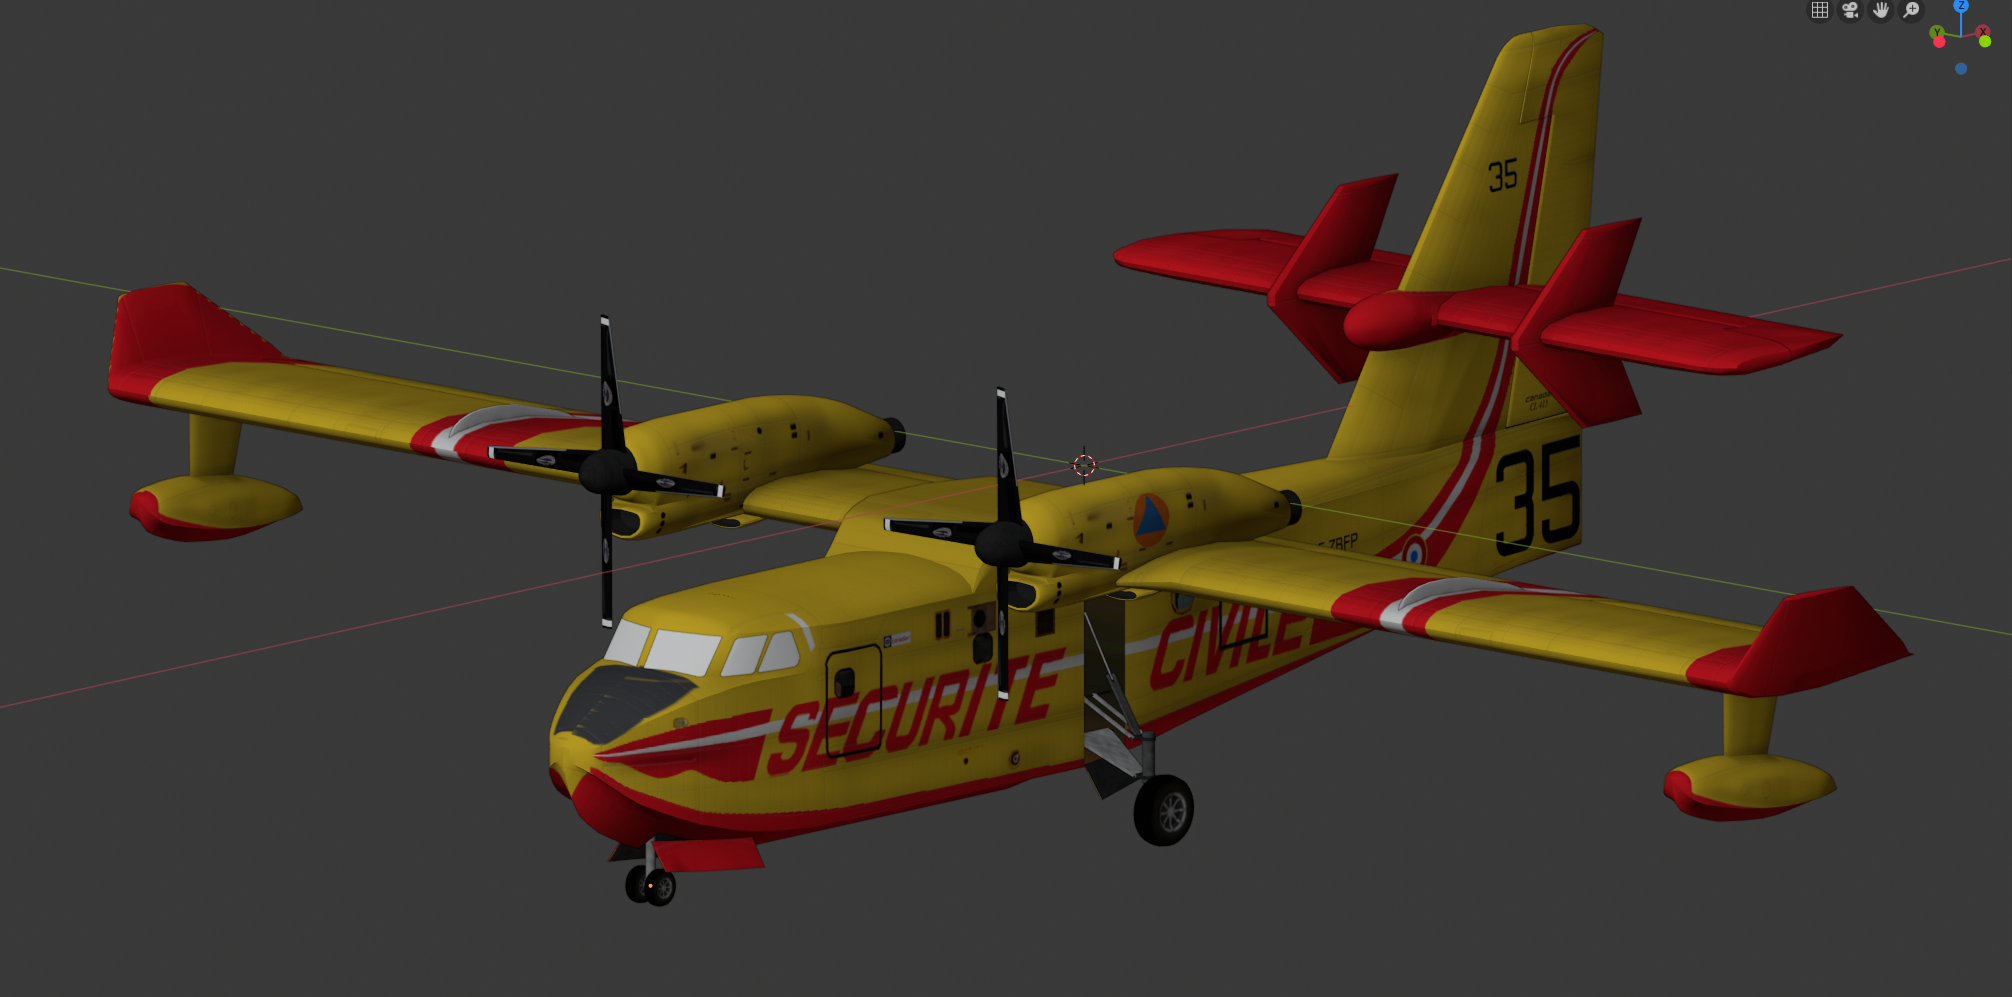
\includegraphics[width=\linewidth]{ImmaginiReport/Canadaircomplete.png}
  \caption{Bombardier-415 opened with Blender v-2.80}
\end{figure}
 
The 3D model of the Bombardier-415\footnote{All the informations about the Bombardier-415 are taken from http://www2.malignani.ud.it/WebEnis/aer/Portfolio/CANADAIR\_CL415.pdf} was downloaded through the site \textit{Cgtrader}\footnote{https://www.cgtrader.com/free-3d-models/aircraft/historic/bombardier-415-superscooper} and then modified using the program Blender v-2.80\footnote{https://www.blender.org/}. The model is composed of 78 children, which compose the torso, the wings, the propellers, the tail and the landing gear. We chose this model because it faithfully reproduces the object we wanted to recreate and it is easily modeled

\begin{lstlisting}[language=Java, caption=Bombardier-415 loader]
GLTFloader.load( 'Models/Bombardier-415/bombardier_canadair.glb', function ( gltf ) {

            model = gltf.scene;
            model.traverse(function (children){
				if ( children instanceof THREE.Mesh ) { children.castShadow = true; }
            });
            if(!light_mode){
                canadair2 = model.clone();
                canadair3 = model.clone();
                canadair2.position.set(-300, 5, -60);
                canadair2.scale.set(1, 1, 1);
                canadair2.rotation.y = Math.PI *  0.5;
                canadair2.castShadow = true;
                scene.add(canadair2);
                canadair3.position.set(-5, 5, 50);
                canadair3.scale.set(1, 1, 1);
                canadair3.rotation.y = -Math.PI *0.5;
                canadair3.castShadow = true;
                scene.add(canadair3);
                aeroporto.push(canadair2);
                aeroporto.push(canadair3);
            }
            model.position.set(10, 4, 9);
            model.scale.set(1, 1, 1);

            // Rename the children
            model.traverse(function (children){

                if (children.name == "heliceG") elica_sx = children;
                if (children.name == "heliceD") elica_dx = children;

                if (children.name == "voletG") flap_int_sx = children;
                if (children.name == "voletD") flap_int_dx = children;

                if (children.name == "aileronG") flap_ext_sx = children;
                if (children.name == "aileronD") flap_ext_dx = children;

                if (children.name == "profondeur") flap_timone = children;
                if (children.name == "direction") timone = children;

                if (children.name == "bolG") bulbo_sx = children;
                if (children.name == "bolD") bulbo_dx = children;

                if (children.name == "porteG") carrello_ant_sx = children;
                if (children.name == "porteD") carrello_ant_dx = children;

                if (children.name == "trappeG") carrello_pst_sx = children;
                if (children.name == "trappeD") carrello_pst_dx = children;

                if (children.name == "roueA") ruote_ant = children;
                if (children.name == "roueG") ruote_pst_sx = children;
                if (children.name == "roueD") ruote_pst_dx = children;

                if (children.name == "axeA") asse_ant = children;

                if (children.name == "axeG1") sospensione_1_sx = children;
                if (children.name == "axeG2") sospensione_2_sx = children;
                if (children.name == "axeG3") sospensione_3_sx = children;
                if (children.name == "axeG4") sospensione_4_sx = children;
                if (children.name == "axeD1") sospensione_1_dx = children;
                if (children.name == "axeD2") sospensione_2_dx = children;
                if (children.name == "axeD3") sospensione_3_dx = children;
                if (children.name == "axeD4") sospensione_4_dx = children;

                if (children.name == "parapG1") supp_carrello_basso_sx = children;
                if (children.name == "parapG2") supp_carrello_alto_sx = children;
                if (children.name == "parapD1") supp_carrello_basso_dx = children;
                if (children.name == "parapD2") supp_carrello_alto_dx = children;

            });
            model.add( camera );
            model.add( particleSys );
            scene.add( model );
        },
        // called while loading is progressing
        function ( xhr ) {
            console.log( ( xhr.loaded / xhr.total * 100 ) + '% loaded' );
        },
        // called when loading has errors
        function ( error ) {
            console.log( 'An error happened' );
        });
\end{lstlisting}

\subsubsection*{World}
The world generates itself autonomously with the advance of the plane so as to make the game lighter and allow to have a more fluid graphics. We decided to generate a forest not too dense, considering the creation of a multitude of trees too heavy and unnecessary for the final purpose of the game. Our goal was to make the idea of an open wooded area. The position of the lake is fixed and is located in front of the runway so as to make immediate his vision. The fire is generated autonomously in a random position within the "work area". The latter is a limited portion of the world within which the plane can move freely, but that, if the player violates the boundaries, produces the failure of the player and consequently the defeat. In this way we were able to create a world limited in space so as to have a light code and prevent the player from getting lost in the infinite immensity of a virtual game.

\subparagraph*{Trees}
We imported the trees from this site. We also decided to manage two different types of trees, a first type is formed by pines\footnote{https://sketchfab.com/3d-models/pine-tree-single-01-ed72511b36c14446a1b596b7e3686d73}, and is the main part of our forest. The other type is generated in the areas affected by the fire and is composed of burnt trees\footnote{https://sketchfab.com/3d-models/tree-free-extra-details-scan-cdb8c99aa5774fcab712f9082b061a9d}. This allows us to make the world more realistic and gives an intuitive idea of the area affected by the fire even when the fire has been extinguished. \\
The trees are loaded in the world dinamically because if we load the entire forest at the beggining of the game the performace will decreace dramatically. The dinamic loading of the forest consist on load only the threes which are in a range around the airplane. 

\subparagraph*{Grass}
For the representation of the grass we decided to reproduce a more detailed type of grass\footnote{https://sketchfab.com/3d-models/yet-another-grass-model-95dc9c01a9ed45a99a3303b95c9f3f91} only when the plane is near the ground (i.e. during the take-off phase). Otherwise, the ground is covered with a "carpet" that gives the idea of a turf in 2D and therefore much lighter. \\
It is positioned only near the airport and also for the grass, as well as trees, the loading in the scene depends on the position of the airplane

\subparagraph*{Fire}
The fire is composed by four orthogonal plane where on each of them is applyed the fire texture. The texture is procedural and it is generated by the shader. We import the shader from the ThreeJS examples. \\
The fire is controlled by three parameters which depend on the difficulty chosen. The parameters are: FireSpeed, FireInitialDimension, FireInterval. The FireInitialDimension is the initial scale of the fire when the game starts, the FireSpeed is the amount of how much the fire increases each time it expands and the FireInterval is how often it expands. Each time it expands its scale grow up by a factor thath depends on the FireSpeed. \\
When the water is dropped over the fire, it will reduce its scale. When it reaches a scale below 0.2 the game is over and you have won.

\subparagraph*{Water}
NON HO IDEA DI COSA SCRIVERE.. VI PREGO PENSATECI VOI (PARTE 2)
lago + scarico acqua + particelle
L'acqua è stata importata da qui\footnote{https://github.com/mrdoob/three.js/blob/master/examples/webgl\_shaders\_ocean.html\#L100}

\subsubsection*{Airport}

\subparagraph*{Hangars}
From the websites \textit{Sketchfab} and \textit{Cgtrader}, we decided to import two different types of hangars so as to give a greater variety to the environment and make the airport area more realistic. The first type of hangar is a closed building\footnote{https://sketchfab.com/3d-models/hangar-558d7e381b9a4b099a49e72ff5824ecb}, very similar to a protected office or warehouse.
The second is the classic hangar\footnote{https://www.cgtrader.com/free-3d-models/military/other/aircraft-low-poly-shelter-hangar} inside the airports, a metal structure that serves to cover the aircraft from the rain and sun. A control tower\footnote{https://open3dmodel.com/download/communication-tower-building\_12469.html} has been positioned next to the hangars for communication with the base.
Hangars, as well as trees, have a dynamic loading. They are loaded in the scene only when they enter in the field of view of the airplane.

\subparagraph*{Take-off Runway}
The runway was imported by \textit{Sketchfab}\footnote{https://sketchfab.com/3d-models/sidewalk-c4d846ab2beb40e09582ef5d93746e6a} and was designed to allow the aircraft to reach a speed of about 215 km/h. Considering that the stall speed of a Bombardier-415 is about 150 km/h and that therefore it must be the minimum speed to face a takeoff, the runway has been designed long enough to allow the possibility of a safe takeoff. We have also chosen to position the runway in the direction of the lake so as to help the player to reach the water surface as quickly as possible. 

\newpage
\section*{Animations of the plane}

\begin{figure}[h!]
  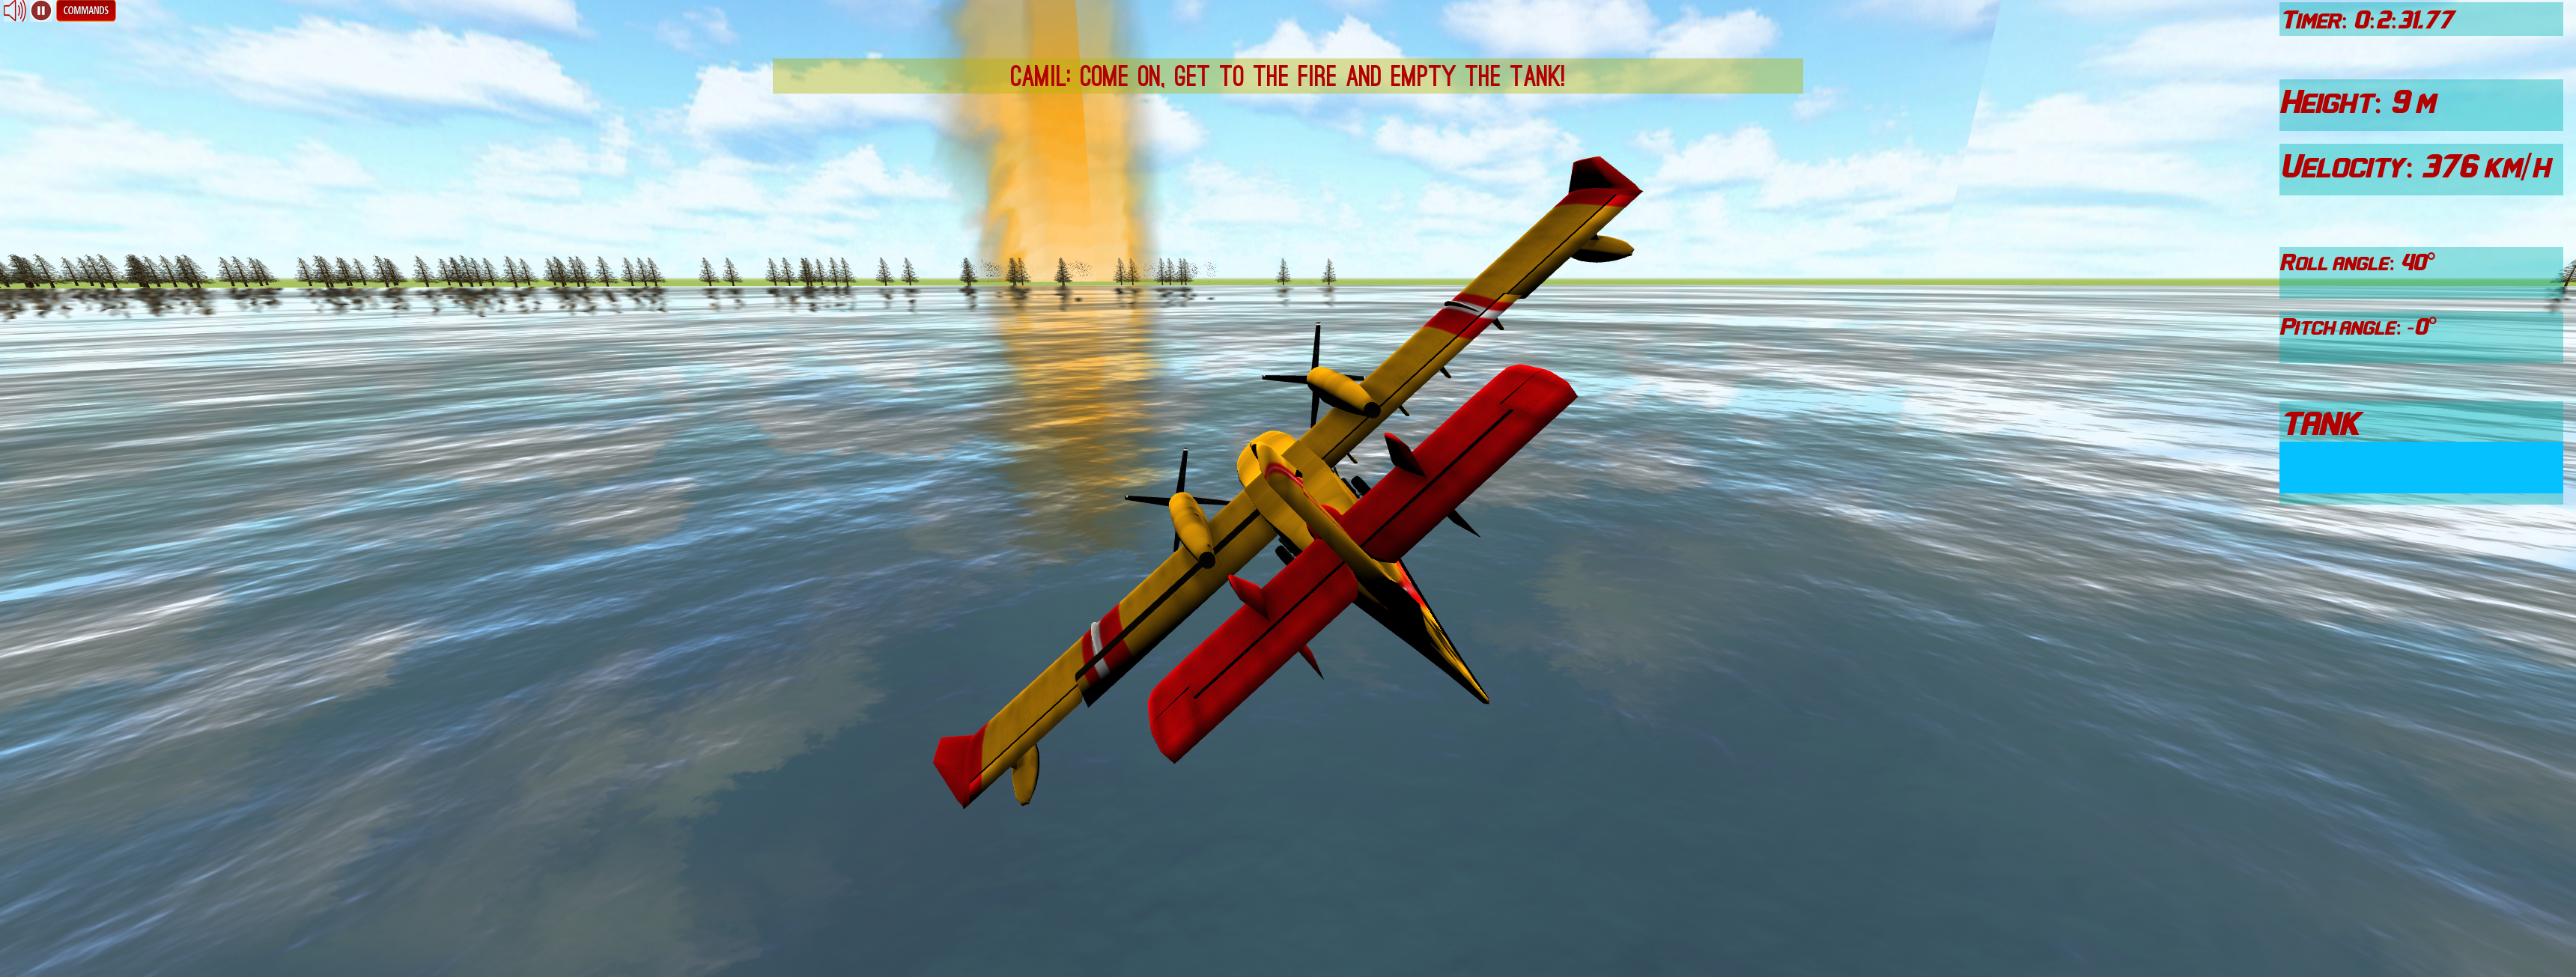
\includegraphics[width=\linewidth]{ImmaginiReport/schermata.png}
  \caption{A screenshot during the game}
\end{figure}

\subsection*{Maneuverability}
Although we had initially decided to make the piloting of the aircraft very similar to a real simulation, with time and several tests we realized that the piloting was extremely complicated for a player without aeronautical knowledge. This problem of piloting would be boundless in the absence of fun, the primary objective of the game, and as a result we decided to structure the piloting in a simpler and more intuitive way. We rely on the WASD command set for piloting, i.e. controlling roll\footnote{The roll angle is the angle that rotates around the longitudinal axis, that is, the axis that connects the tip with the tail.} and pitch\footnote{The pitch angle is the angle that rotates along the latitudinal axis, that is, the axis that connects the two wing ends.} angles. We decided to avoid rotations along the yaw axis because we integrated the movements along this axis in the (automatic) movements of the rudder, which moves according to the turn to counteract the phenomenon of adverse yaw\footnote{https://en.wikipedia.org/wiki/Adverse\_yaw}. To turn, the player simply press the A (left) or D (right) commands. Pressing one of these two commands will cause the player to rotate along the roll axis in the direction of the turn, lowering the internal flaps of the internal wing and slightly raising the internal flaps of the external wing to the rotation. This movement of the flaps allows the inclination of the plane, in fact the flaps of the inner wing, slowing down cause an effect of inertia which rotates the plane, however, being the inner wing braked by the flaps, it is necessary to raise slightly the flaps of the outer wing so as to have a slowdown in the rotation of the anode the axis of yaw, also controlled by the movement of the rudder. All of these actions cause the plane to tilt and turn. For simplicity we have decided to limit the rotation up to a roll angle of 90 degrees. The rotation is progressive and depends on the angle of roll, the more the inclination will be accentuated and the smaller the turning radius will be. On the right of the screen, there will be a roll angle indicator expressed in degrees, positive for counterclockwise rotations and negative for clockwise rotations. Rotation along the pitch axis is controlled by the W controls for the dive and the S controls for the cab. Also in this case the rotation is limited and less than 60 degrees. During pitch rotation, the outer flaps of the wings move in a coordinated and inverse manner to the rudder flaps. In fact, for the cabin you will need to raise the front of the aircraft and lower the thing. To do this, the outer flaps of the wings will be lowered progressively, while the rudder flaps will be raised, thus causing a depression and lowering the tail. During the dive the opposite happens, i.e. the outer flaps of the wings are raised, while the rudder flaps are lowered. As for the roll, also the pitch has an indicator of the rotation, positive during the dive and negative during the cab. We decided not to give the possibility to mix the roll and pitch angles as the player would face configurations of difficult interpretation. We thought of a self-stable profile, which is for both roll and pitch, once released the command, the aircraft will return independently in the stable configuration. This greatly simplifies maneuverability and makes the game more accessible.

\newpage

\begin{lstlisting}[language=Java, caption=Manage commands]
document.addEventListener("keydown", onDocumentKeyDown, false);
function onDocumentKeyDown(event) {

    if (!playFlag) return;

    switch (event.keyCode) {
        case 77: // m
            if (motors == 0) {
                motors = 1;
                speed_helic = 0.05;
                engine = setInterval(go_motors, 1);
                //sound on
                motor_sound.sound.play();
                setInterval(motion, 1);
                setInterval(manage_velocity, 40);
            }
            break;
        case 66: // b
            clearInterval(reset);
            flag = false;
            if (motors != 0 && motors != 5) {
                motors += 1;
                speed_helic += 0.05;
                motor_sound.sound.playbackRate += .7;
            }
            if (weels != 5) {
                weels += 1;
                speed_weels += 0.1;
            }
            break;
        case 78: // n
            clearInterval(reset);
            flag = false;
            if (motors != 0 && motors != 1) {
                motors -= 1;
                speed_helic -= 0.05;
                motor_sound.sound.playbackRate -= .7;
            }
            break;
        case 65: // a
            if (pitch < 0.05 && pitch > -0.05 && roll <= 90 && !ground && !emptyingTank && !onLake) {
                clearInterval(reset);
                flag = false;
                model.rotateX(Math.PI / 300);
                roll += 180 / 300;
            }
            break;
        case 68: // d
            if (pitch < 0.05 && pitch > -0.05 && roll >= -90 && !ground && !emptyingTank && !onLake) {
                clearInterval(reset);
                flag = false;
                model.rotateX(-Math.PI / 300);
                roll -= 180 / 300;
            }
            break;
        case 87: // w
            if (roll < 0.05 && roll > -0.05 && pitch <= 60 && !emptyingTank && !onLake && !ground) {
                clearInterval(reset);
                flag = false;
                model.rotateZ(Math.PI / 400);
                pitch += 180 / 400;
            }
            break;
        case 83: // s
            if (roll < 0.05 && roll > -0.05 && pitch >= -60 && !emptyingTank && (!ground || vel > 150)) {
                clearInterval(reset);
                flag = false;
                model.rotateZ(-Math.PI / 400);
                pitch -= 180 / 400;
            }
            break;
        case 67: // c
            if (carrello && !ground) {
                t = 0;
                s = 0;
                carrello = false;
                pressed_c = true;
                cart_sound.sound.play();
                setInterval(close_doors_ant, 10);
                setInterval(close_doors_back, 10);
            }
            break;
        case 32: //space bar
            if (tank) {
                let timeout;
                pressed_bar = true;
                let r = roll.toFixed(0);
                let p = pitch.toFixed(0);
                if (r > -20 && r < 20 && p > -40 && p < 80 && (!onLake || height > height_difficulty)) {
                    waterClock.start();
                    tank = false;
                    emptyingTank = true;
                    water_sound.sound.play();
                    moving_bar(0);
                }
                if(posizione_sopra_fuoco(model.position.x,model.position.z)){
                    var distanzaDaFuoco = Math.sqrt(Math.pow((model.position.x - firePosition[0]),2)
                        + Math.pow(model.position.z - firePosition[1],2));
                    var quanto = 5 - Math.abs(distanzaDaFuoco)/100;
                    if(quanto < 0)
                        quanto = 1;
                    console.log(quanto);
                    fire_extinguish(quanto);
                    msg_id++;
                    if (msg_id%3==0) msg_id=0;
                }
                clearTimeout(timeout);
                timeout = setTimeout(function() {
                pressed_bar = false; 
                }, 5000);
            } else if (onLake && !emptyingTank) {
                moving_bar(1);
                tank = true;
            }
            break;
    }
};
\end{lstlisting}
 

\subsection*{Velocity}
We have decided to equip the plane with five levels of speed. Initially it starts from a zero speed, with the engines off. Pressing the M button starts the engines, which causes the wheels to start (both front and rear) and the propellers to rotate (the rotation takes place in the opposite direction to prevent the aircraft from rotating due to the moment of inertia). Once the motors have been switched on, the speed can be controlled using keys B and N, which allow acceleration and deceleration respectively. Each time one of the two keys is pressed, the next (or previous) speed level is reached, up to a maximum level of 5 and a minimum level of 1. The speeds for each level are the following:
\begin{itemize}
\item \textbf{Level 1}: 171 Km/h
\item \textbf{Level 2}: 206 Km/h
\item \textbf{Level 3}: 263 Km/h
\item \textbf{Level 4}: 320 Km/h
\item \textbf{Level 5}: 376 Km/h
\end{itemize}
However, speeds are affected by the aircraft's trim, reducing in the case of a cab or increasing in the case of a dive. This was achieved by integrating the pitch angle into the manage\_velocity function.

\begin{lstlisting}[language=Java, caption=Function manage\_velocity]
function manage_velocity() {

    if (!playFlag) return;

    if (ground && motors > 0 && vel < 171) vel += 1.2;
    if (vel < 206+(Math.sin(pitch*Math.PI/180)*20) && motors > 1) vel += 0.67;
    else if (vel < 263+(Math.sin(pitch*Math.PI/180)*20) && motors > 2) vel += 0.5; 
    else if (vel < 320+(Math.sin(pitch*Math.PI/180)*20) && motors > 3) vel += 0.5; 
    else if (vel < 376+(Math.sin(pitch*Math.PI/180)*20) && motors > 4) vel += 0.33; 

    else if (vel > 376+(Math.sin(pitch*Math.PI/180)*20)) vel -= 0.5; 
    else if (vel > 320+(Math.sin(pitch*Math.PI/180)*20) && motors < 5) vel -= 0.5;
    else if (vel > 263+(Math.sin(pitch*Math.PI/180)*20) && motors < 4) vel -= 0.5;
    else if (vel > 206+(Math.sin(pitch*Math.PI/180)*20) && motors < 3) vel -= 0.5;
    else if (vel > 171+(Math.sin(pitch*Math.PI/180)*20) && motors < 2) vel -= 0.5;

    height = model.position.y*0.4;

}
\end{lstlisting}

\subsection*{Take-off}
The take-off phase is one of the most delicate phases in the flight activity, the pilot must make the plane take as much speed as possible and then cabrate to take altitude. To make the take-off phase easier, we have prevented the player from making a dive or a turn during the initial take-off phase. This was possible thanks to the ground variable, a Boolean variable that is true when the aircraft is on the ground. A Bombardier-415 has a stall speed of about 150 km/h, so we made it impossible for the plane to take off at lower speeds. Being on the runway, in addition to the thrust of the propellers also has the acceleration due to the rotation of the wheels, so the acceleration during the ground phase of the takeoff is greater than that which occurs during the flight. Once the take-off is complete, it is essential that the pilot calls back the landing gear, especially as the landing gear would crash if it approached an aquatic surface. To close the landing gear, the player can press button C, which will activate two functions for closing the front and rear landing gear. 

\begin{figure}[h!]
  \centering
  \begin{subfigure}[b]{0.4\linewidth}
    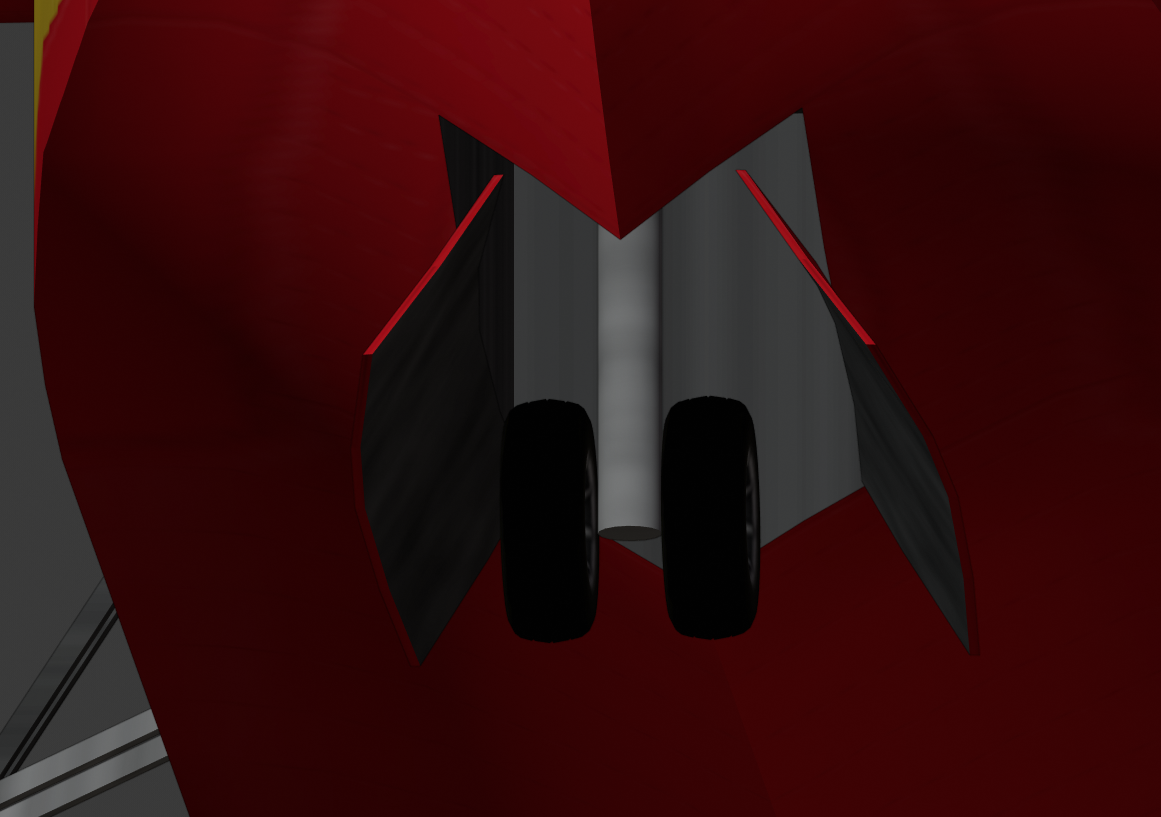
\includegraphics[height=48mm]{ImmaginiReport/antopen.png}
    \caption{Front gear open}
  \end{subfigure}
  \begin{subfigure}[b]{0.4\linewidth}
    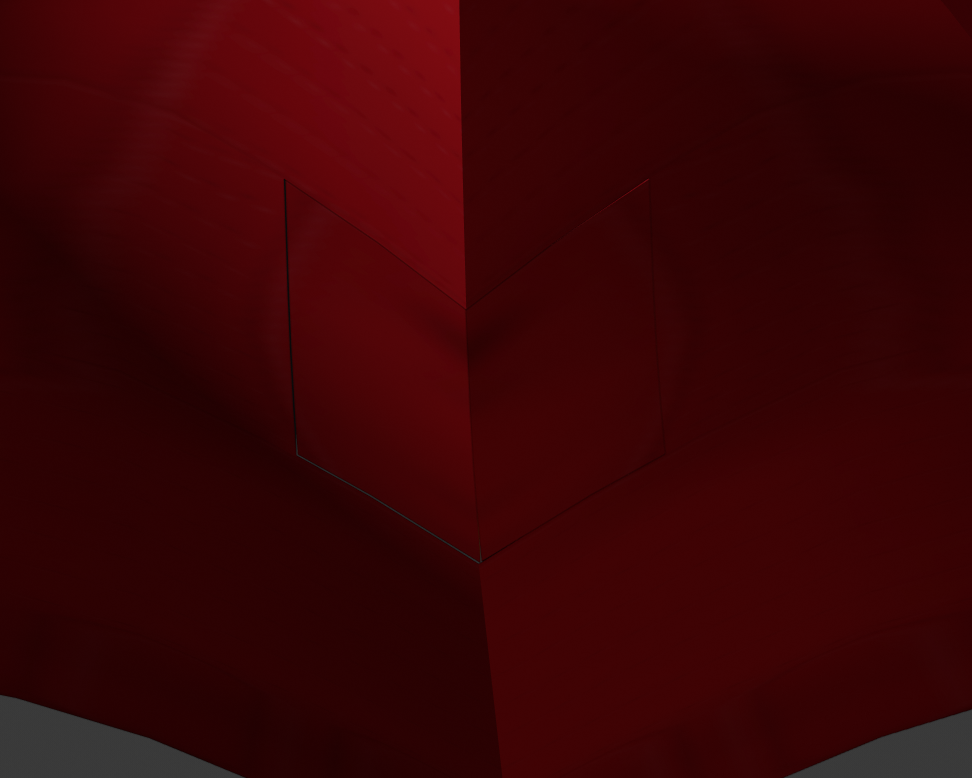
\includegraphics[height=48mm]{ImmaginiReport/antclose.png}
    \caption{Front gear close}
  \end{subfigure}
  \caption{Front gear during the closing of the landing gears}
\end{figure}

\begin{figure}[h!]
  \centering
  \begin{subfigure}[h!]{0.4\linewidth}
    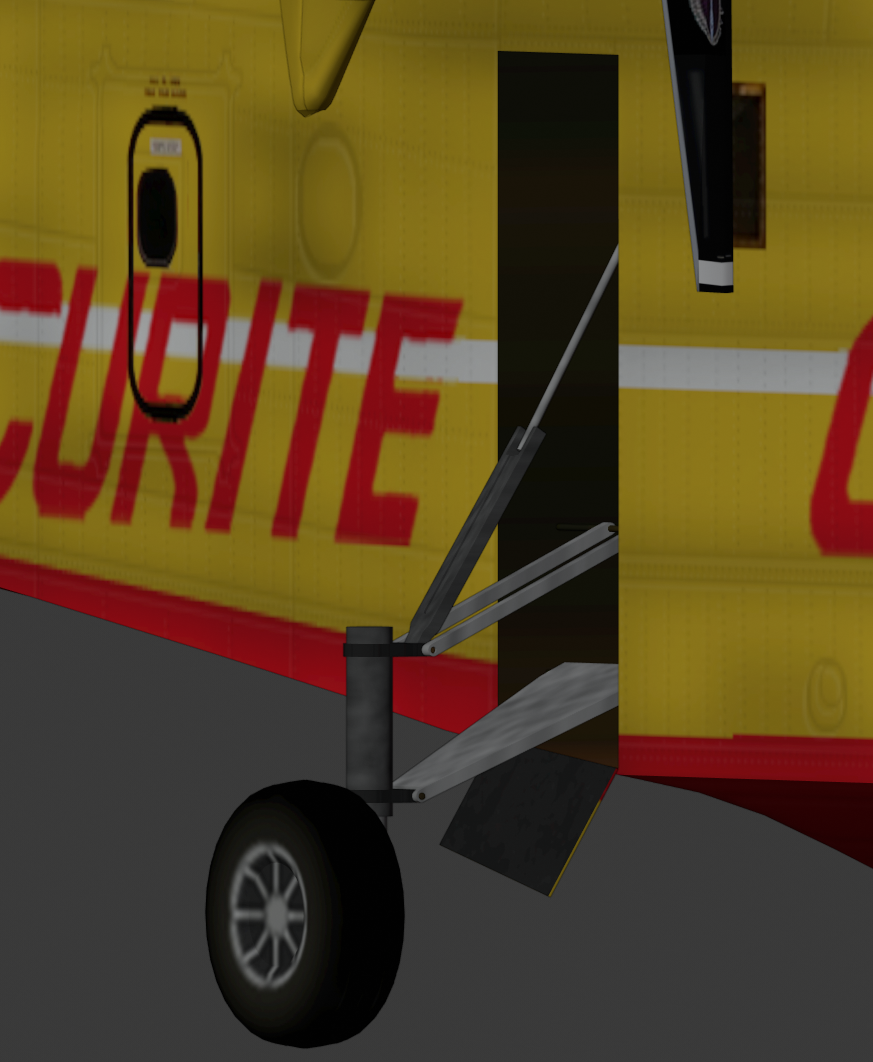
\includegraphics[height=80mm]{ImmaginiReport/postopen.png}
    \caption{Rear gear open}
  \end{subfigure}
  \begin{subfigure}[h!]{0.4\linewidth}
    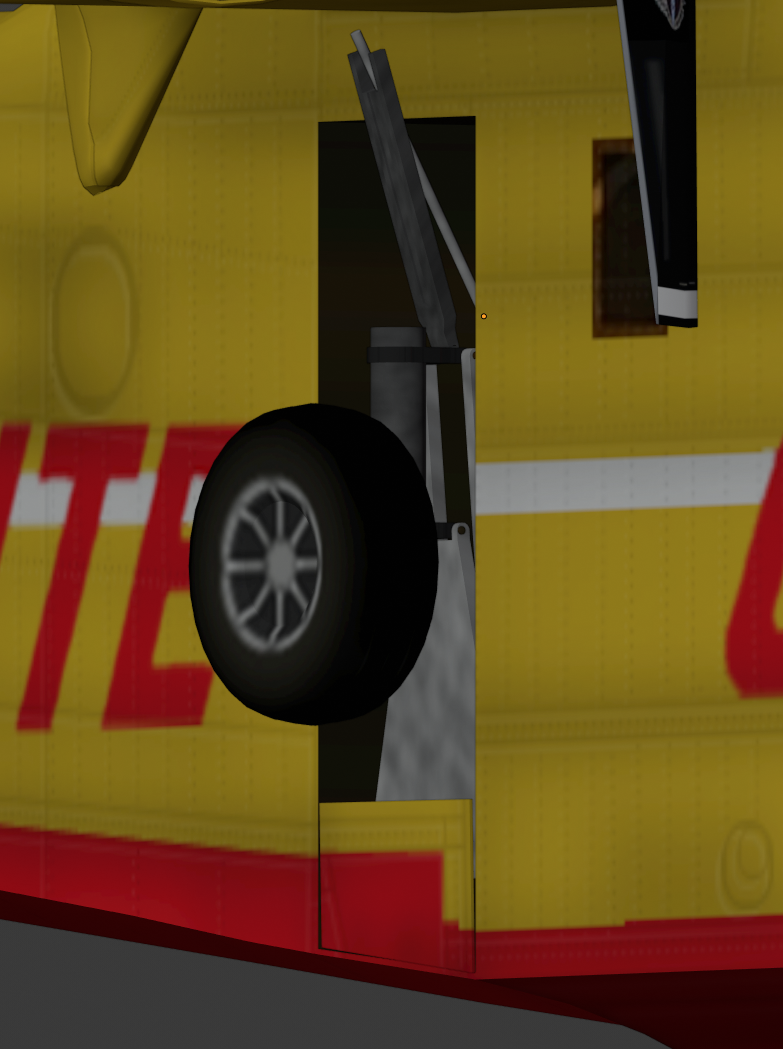
\includegraphics[height=80mm]{ImmaginiReport/postclose.png}
    \caption{Rear gear close}
  \end{subfigure}
  \caption{Rear gear during the closing of the landing gears}
\end{figure}

\newpage
\section*{Home Page}

\begin{figure}[h]
  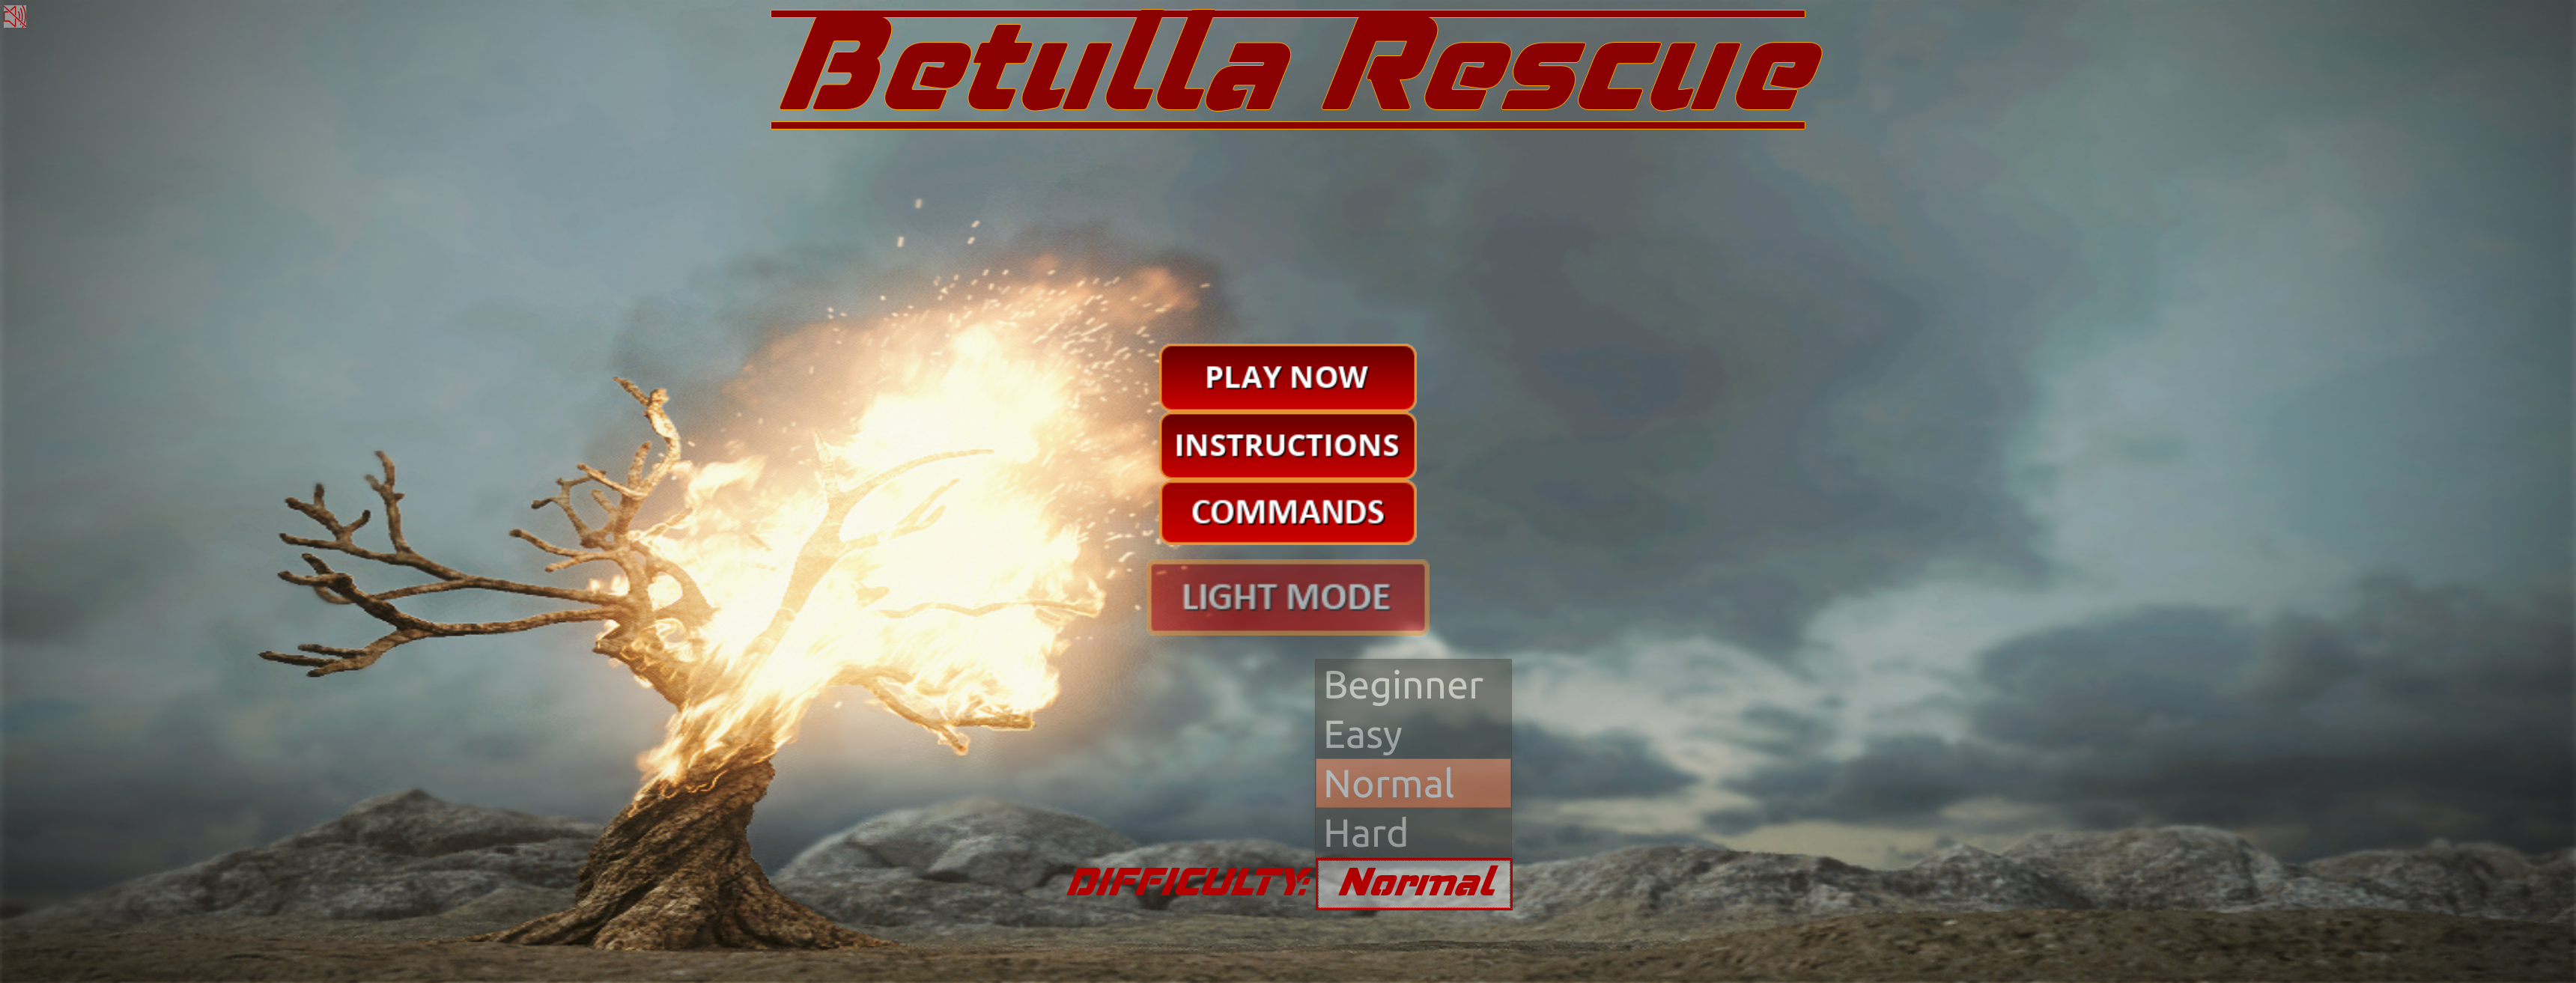
\includegraphics[width=\linewidth]{ImmaginiReport/initial.png}
  \caption{Home page and with diccoulty menu}
\end{figure}

The home page has 4 buttons in the middle of the screen: 
\begin{itemize}
\item \textbf{PLAY GAME}: allows you to start the game.
\item \textbf{INSTRUCTIONS}: provides a detailed explanation of the rules and commands.
\item \textbf{COMMANDS}: illustrates the functions associated with the keys.
\item \textbf{LIGHT MODE}: activates the light mode required for less powerful devices.
\end{itemize}
At the bottom you can adjust the difficulty, choosing through 4 levels that appear from a drop-down menu. The difficulties are as follows:
\begin{itemize}
\item \textbf{BEGINNER}: to be considered as a tutorial, the fire will not expand and you can fill the tank with a height less than or equal to 15 meters.
\item \textbf{EASY}: For novice players, the fire will expand slowly and you can fill the tank with an altitude less than or equal to 10 meters.
\item \textbf{NORMAL}: For players looking for a challenge, the fire will expand quickly and you can fill the tank with an altitude less than or equal to 6 meters.
\item \textbf{HARD}: For experienced players who want an extreme challenge, the fire will expand very quickly and you can fill the tank with an altitude less than or equal to 3 meters.
\end{itemize}
At the top left of the home screen there is a button with a loudspeaker that allows you to enable or disable the sound.

\subsection*{Loading window}
During the most intense uploads we have inserted a screen that gives an idea of the loading situation. The screen was downloaded from \textit{Freefrontend}\footnote{https://freefrontend.com/css-loaders/}, we chose a simple screen that reflected the colors of the fire\footnote{https://codepen.io/sashatran/pen/vRrxXw}. We wrote the following code to upload it:

\begin{lstlisting}[language=Java, caption=Loading manager]
const loadingManager = new THREE.LoadingManager( () => {
    
        const loadingScreen = document.getElementById( 'loading-screen' );
        loadingScreen.classList.add( 'fade-out' );
        loadingScreen.style.display = "none";
        loadingScreen.classList.remove( 'fade-out' );

        menu_music.muted = true;
        
        //show game window
        document.getElementById('game_id').style.display = 'block';

        if (volume) fire_sound.setVolume( 8 );
        else fire_sound.setVolume( 0 );

        playFlag = true;
        animate();
        setInterval(messages, 1000);
        startTime=clock.getElapsedTime();
        
        // optional: remove loader from DOM via event listener
        loadingScreen.addEventListener( 'transitionend', onTransitionEnd );
        
} );
\end{lstlisting}

\subsection*{Audio}
We imported several audio tracks to reproduce the most common sounds. The noise of the motors\footnote{https://freesound.org/people/craigsmith/sounds/438650/} is activated when the M button is pressed and increases or decreases the frequency as the speed increases or decreases. This gives a good idea of acceleration or deceleration. To close the landing gear we relied on an audio track\footnote{https://freesound.org/people/77Pacer/sounds/425273/} slowing down the playback to synchronize the sound with the our  landing gear closing time. For the fire, we relied on a specific track\footnote{https://freesound.org/people/Fraho uctalStudios/sounds/363092/} to reproduce the noise of the fire. In the same way, the sound of a waterfall\footnote{https://freesound.org/people/InspectorJ/sounds/365921/} is reproduced each time the plane empties the tank. We decided to also insert a background music track\footnote{https://www.bensound.com/royalty-free-music/track/badass} during the initial screen and several mini-tracks to accompany the victory\footnote{http://www.orangefreesounds.com/winning-sound-effect/} or game over screen\footnote{https://freesound.org/people/themusicalnomad/sounds/253886/}. 


\end{document}
